\def\difficulty{1}
\sujet{Shape From Focus}
\index{Shape From Focus}

\label{lbl:tutorial:sff}
\begin{note}This tutorial introduces the basic shape from focus concepts. The objective is to reconstruct a focused image from a serie (generally a stack) of images with inhomogene focus (see Fig. \ref{fig:stack}).\end{note}

\begin{figure}[htbp]
\centering\caption{Different images of the stack, from a corneal endothelium in optical microscopy (with 3D microscope).}%
 \subfloat[Layer 1]{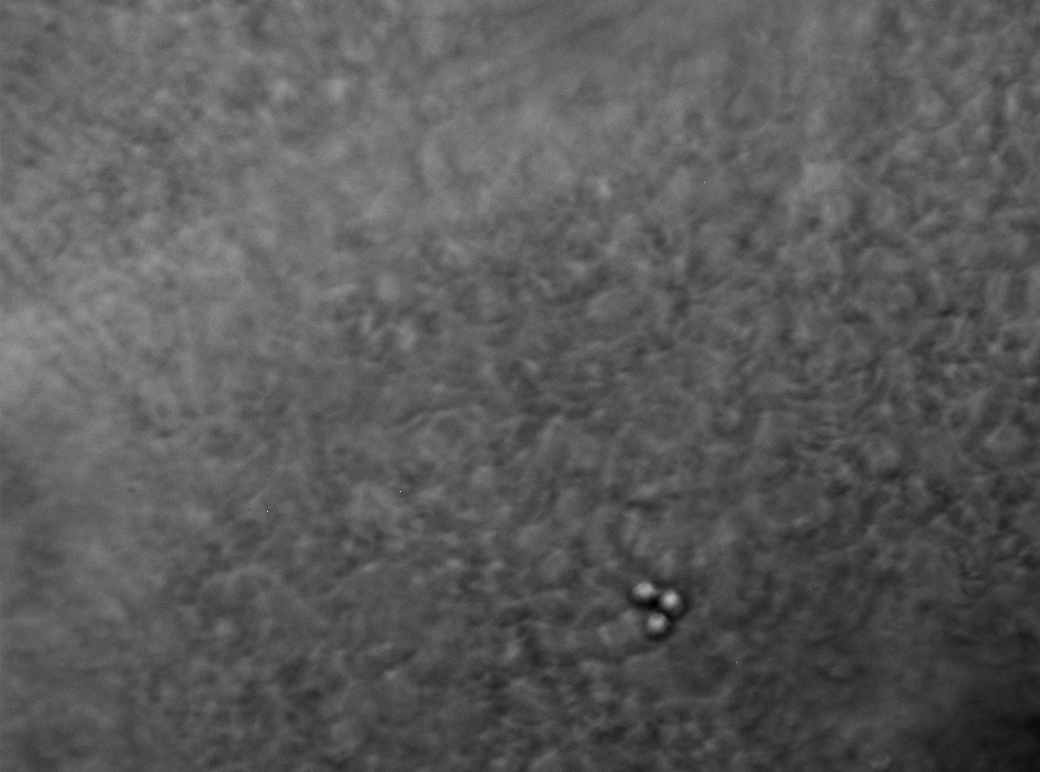
\includegraphics[width=.45\linewidth]{Couche_1.png}}
 \hfill
 \subfloat[Layer 9]{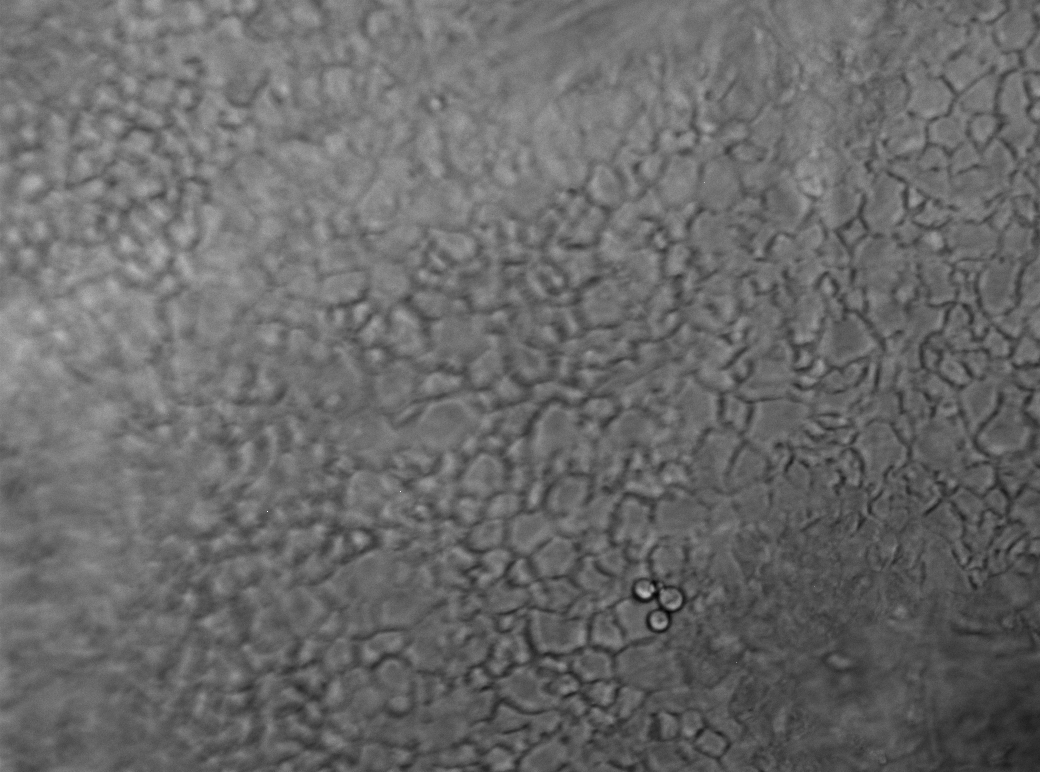
\includegraphics[width=.45\linewidth]{Couche_9.png}}
 
 \subfloat[Layer 18]{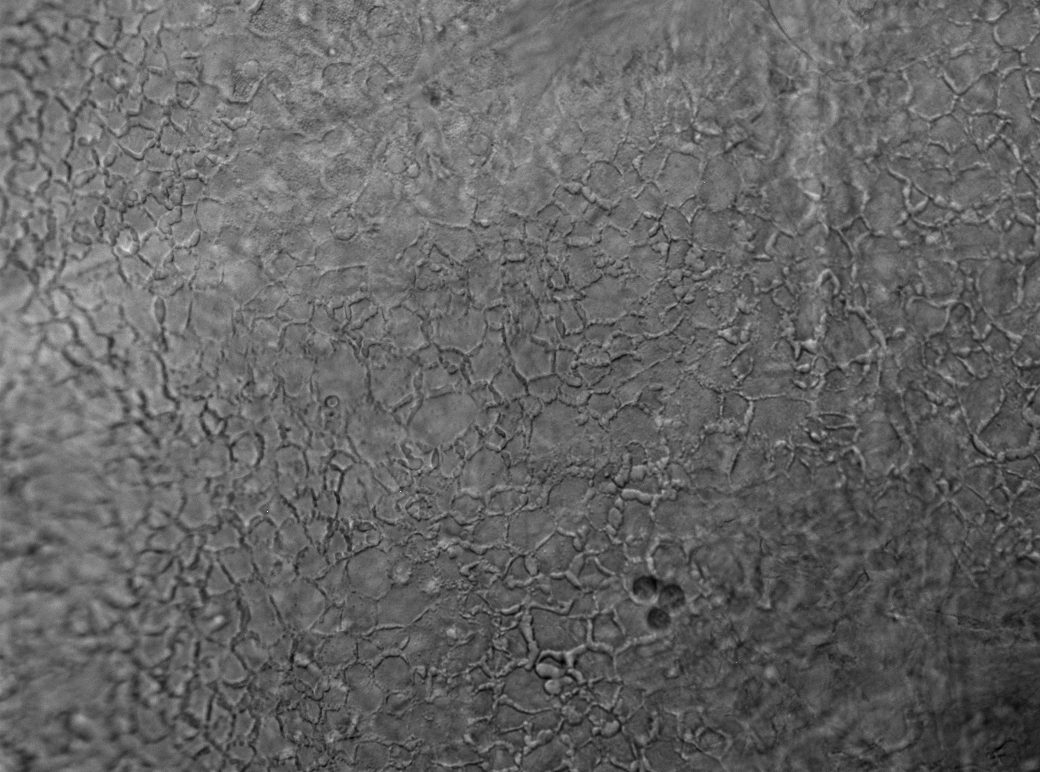
\includegraphics[width=.45\linewidth]{Couche_18.png}}\hfill
 \subfloat[Layer 24]{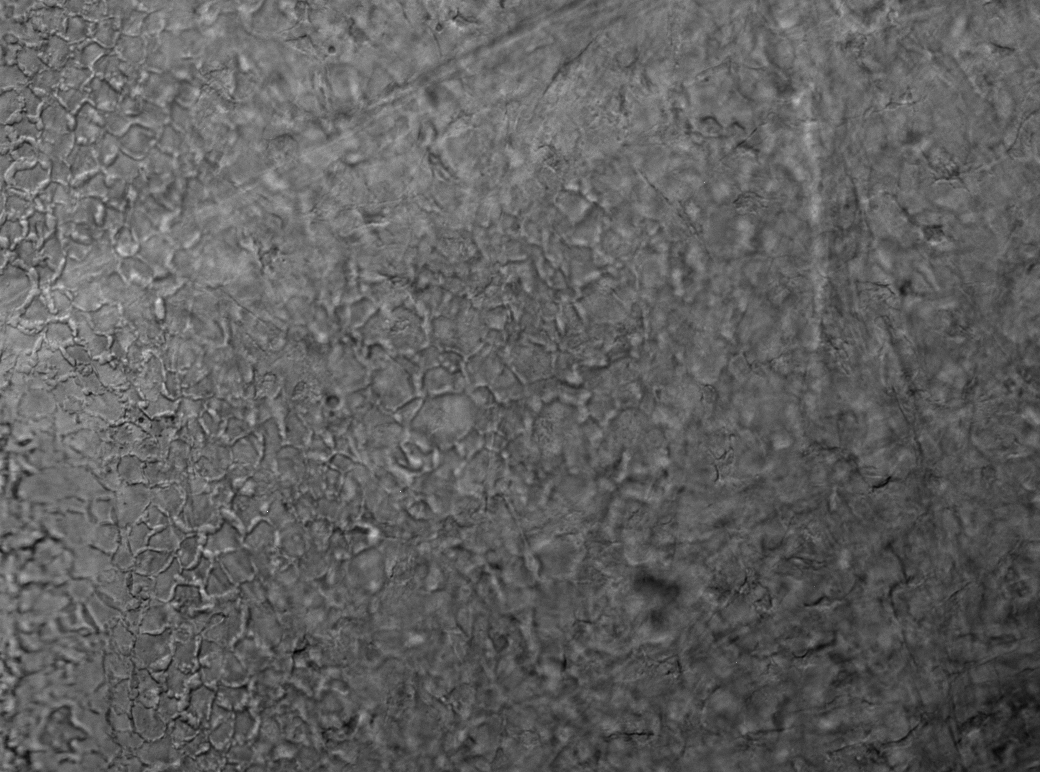
\includegraphics[width=.45\linewidth]{Couche_24.png}}%
 \label{fig:stack}%
\end{figure}


\section{Introduction to classical methods}
An optic system has a limited depth of field. When observing non plane surfaces with a microscope, some parts of the observation may be blurred as well as some others may be correctly focused. 

To overcome this problem and reconstruct an all-focused image as well as a surface (see Fig. \ref{fig:surface}), an algorithm will look at every pixel of the images in the stack and select the most focused one, by the way of a focus measure. This tutorial proposes to test some classical focus measures. You can have a look at \cite{Fernandes2010} and \cite{Fernandes2012} to see real applications.

\begin{figure}[htbp]
\centering\caption{Reconstruction of the surface and the texture.}%
\vspace*{1pt}%
 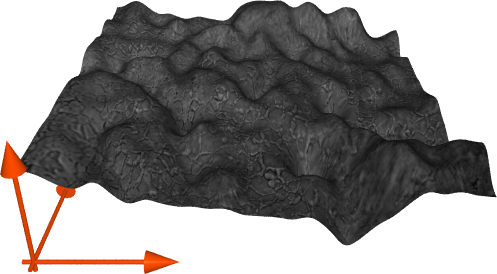
\includegraphics[width=0.75\linewidth]{meshc.png}%
 \vspace*{1pt}%
 \label{fig:surface}%
\end{figure}


Practically, TIF files can handle stacks of images. Here is a way to open such a file:



\begin{python}
from skimage import io

I = io.imread('volume.tif');
I = I.astype('float');
\end{python}


\begin{matlab}
% load a stack of images in file
info = imfinfo(stackfile);
num_images = numel(info);
% store the images into stack 
stack=zeros(info(1).Height, info(1).Width, num_images);
for k = 1:num_images
    stack(:,:,k)=imread(stackfile, k);
    % you can now do something with each image
end
\end{matlab}

In the following, each of the proposed methods will compute a focus measure layer by layer, and will maximize this measure over the stack to find the most focused layer. 

\subsection{Sum of Modified Laplacian}
\index{Shape From Focus!SML}
One of the first methods had been proposed by \cite{Nayar1994}. It is based on the second derivatives, specifically the Laplacian operator:
$$\bigtriangleup^2 I = \frac{\partial^2 I}{\partial x^2} + \frac{\partial^2 I}{\partial y^2}$$

The problem with this operator is that the second derivatives in the x and y dimensions can have opposite signs. One way to overcome this problem is to introduce the modified Laplacian as follows:
$$\bigtriangleup_M^2 I = \left|\frac{\partial^2 I}{\partial x^2}\right| + \left|\frac{\partial^2 I}{\partial y^2}\right|$$

The discrete approximation of the modified Laplacian is computed as:
\begin{multline}ML(x, y)= \left| 2I(x,y)-I(x-1, y)-I(x+1,y)\right| \\
+ \left| 2I(x,y)-I(x, y-1)-I(x,y+1)\right|
\end{multline}
                                                                                                             

Then, the focus measure based on the modified Laplacian is:
$$F_{ML} = \displaystyle{\sum_{(x,y)\in\omega}}ML(x,y)$$

\subsection{Variance}
\index{Shape From Focus!Variance}
The measure of focus based on the variance is today the mainly used method \cite{Groen1985,Sugimoto1985}. It is based on the computation of the variance in a window $\omega$, with $N=\#\omega$ being the size of the window:
$$F_v=\displaystyle{\sum_\omega} \left( I -\underbrace{\frac{1}{\#\omega} \displaystyle{\sum_\omega} I}_{\textrm{Mean of I}}\right)^2$$

\subsection{Tenengrad}
\index{Shape From Focus!Tenengrade}
In \cite{Krotkov1988}, we can find the definition of the tenengrad \cite{Tenenbaum1970}. Let $S(x,y)$ be the norm of the Sobel gradient of image $I$.
$$F_t(I)=\displaystyle\sum_\omega S^2$$
Notice that the original definition requires a threshold value that requires heuristic choices, which is out of the topic of this tutorial.

\subsection{Variance of Tenengrad}
\index{Shape From Focus!Variance of Tenengrad}
 We define the variance of Tenengrad measure of focus by:
$$F_{vt}(I)=F_v(S)$$.

\section{Texture and surface reconstruction}
\begin{qbox}
A set of images (Vickers indentation test \cite{Fernandes2010}, and a human corneal endothelium \cite{Fernandes2012}) are proposed.
For all the detailed methods:
\begin{itemize}
 \item reconstruct the surface and the texture of the image (an image focused on its all field of view).

\end{itemize}

\end{qbox}

\subsection{Open question}
\begin{qbox}
Several methods have been implemented in order to perform the 3D surface/texture reconstruction. Propose a numerical measure that could compare the results and measure the effciciency of these methods? What is the best method?
\end{qbox}


